\begin{figure}[H]
    \centering
    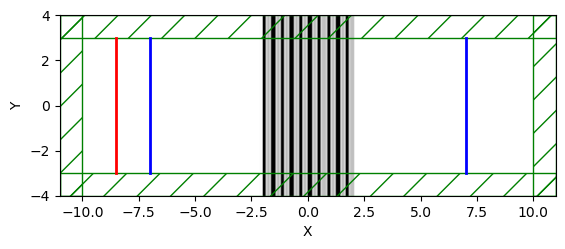
\includegraphics[width=0.8\linewidth]{Figures/bragg_design.png}
    \caption{}
    \label{fig:bragg_design}
\end{figure}

\begin{figure}[H]
    \centering
    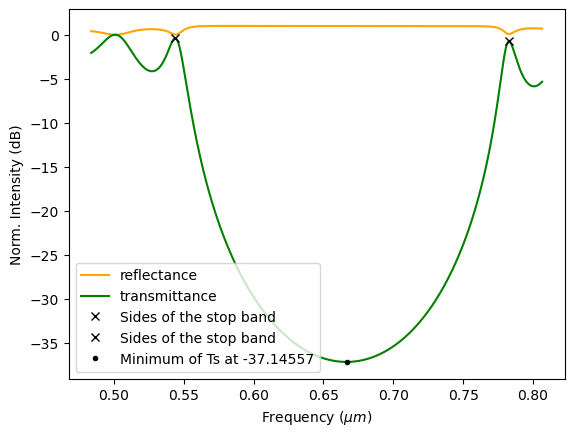
\includegraphics[width=0.6\linewidth]{Figures/bragg_spectrum.png}
    \caption{}
    \label{fig:bragg_spectrum}
\end{figure}

\begin{figure}[H]
    \centering
    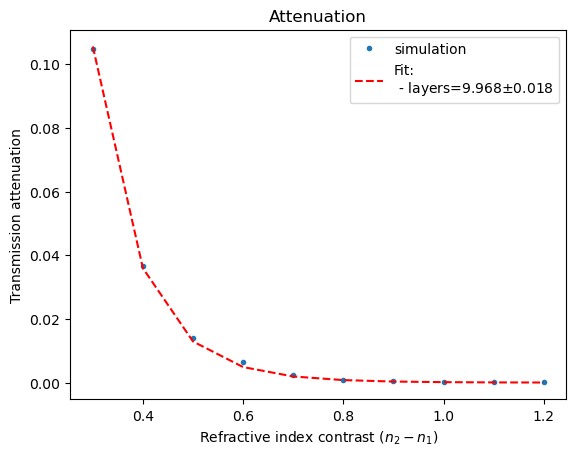
\includegraphics[width=0.6\linewidth]{Figures/bragg_attenuation_vs_index.png}
    \caption{}
    \label{fig:bragg_attenuation_vs_index}
\end{figure}

\begin{figure}[H]
    \centering
    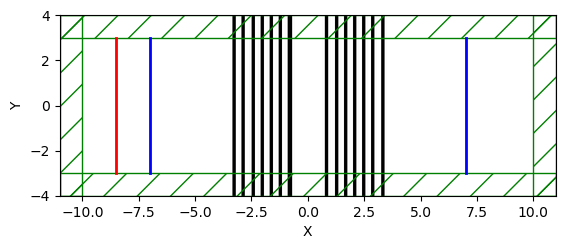
\includegraphics[width=0.8\linewidth]{Figures/bragg_cavity_design.png}
    \caption{}
    \label{fig:bragg_cavity_design}
\end{figure}

\begin{figure}[H]
    \centering
    \begin{subfigure}[b]{0.45\linewidth}
        \centering
        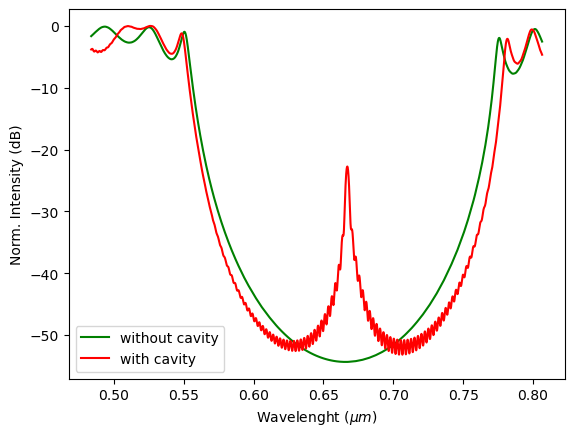
\includegraphics[width=\linewidth]{Figures/bragg_vs_cavity_spectrum.png}
        \caption{}
        \label{fig:bragg_vs_cavity_spectrum}
    \end{subfigure}
    \hfill
    \begin{subfigure}[b]{0.45\linewidth}
        \centering
        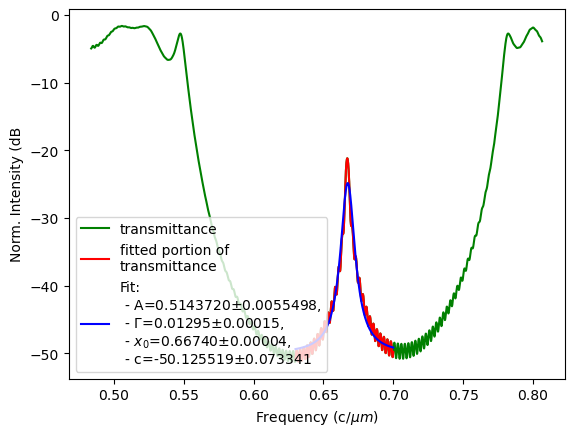
\includegraphics[width=\linewidth]{Figures/bragg_cavity_spectrum_fit.png}
        \caption{}
        \label{fig:bragg_cavity_spectrum_fit}
    \end{subfigure}
\end{figure}

\begin{figure}[H]
    \centering
    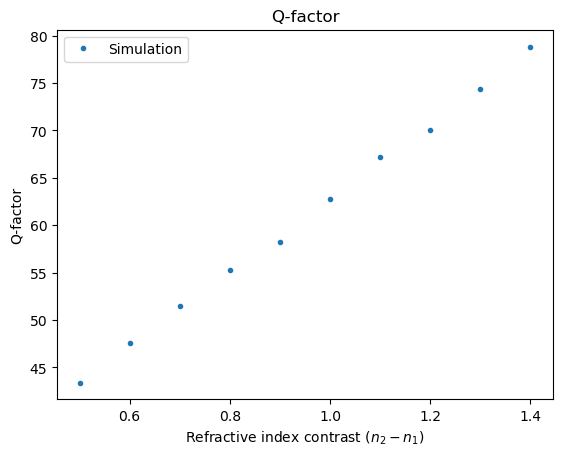
\includegraphics[width=0.6\linewidth]{Figures/bragg_cavity_qfactor_vs_index.png}
    \caption{}
    \label{fig:bragg_cavity_qfactor_vs_index}
\end{figure}